%%%%%%%%%%%%%%%%%%%%%%%%%%%%%%%%%%%%%%%%%
% Short Sectioned Assignment
% LaTeX Template
% Version 1.0 (5/5/12)
%
% This template has been downloaded from:
% http://www.LaTeXTemplates.com
%
% Original author:
% Frits Wenneker (http://www.howtotex.com)
%
% License:
% CC BY-NC-SA 3.0 (http://creativecommons.org/licenses/by-nc-sa/3.0/)
%
%%%%%%%%%%%%%%%%%%%%%%%%%%%%%%%%%%%%%%%%%

%----------------------------------------------------------------------------------------
%	PACKAGES AND OTHER DOCUMENT CONFIGURATIONS
%----------------------------------------------------------------------------------------

\documentclass[paper=a4, fontsize=11pt]{scrartcl} % A4 paper and 11pt font size

\usepackage[T1]{fontenc} % Use 8-bit encoding that has 256 glyphs
\usepackage{fourier} % Use the Adobe Utopia font for the document - comment this line to return to the LaTeX default
\usepackage[english]{babel} % English language/hyphenation
\usepackage{amsmath,amsfonts,amsthm} % Math packages
\usepackage{graphicx}
\usepackage{verbatim}

\usepackage{geometry}
\usepackage{float}

\usepackage{lipsum} % Used for inserting dummy 'Lorem ipsum' text into the template

\usepackage{sectsty} % Allows customizing section commands
\allsectionsfont{\centering \normalfont\scshape} % Make all sections centered, the default font and small caps

\usepackage{fancyhdr} % Custom headers and footers
\pagestyle{fancyplain} % Makes all pages in the document conform to the custom headers and footers
\fancyhead{} % No page header - if you want one, create it in the same way as the footers below
\fancyfoot[L]{} % Empty left footer
\fancyfoot[C]{} % Empty center footer
\fancyfoot[R]{\thepage} % Page numbering for right footer
\renewcommand{\headrulewidth}{0pt} % Remove header underlines
\renewcommand{\footrulewidth}{0pt} % Remove footer underlines
\setlength{\headheight}{13.6pt} % Customize the height of the header

\numberwithin{equation}{section} % Number equations within sections (i.e. 1.1, 1.2, 2.1, 2.2 instead of 1, 2, 3, 4)
\numberwithin{figure}{section} % Number figures within sections (i.e. 1.1, 1.2, 2.1, 2.2 instead of 1, 2, 3, 4)
\numberwithin{table}{section} % Number tables within sections (i.e. 1.1, 1.2, 2.1, 2.2 instead of 1, 2, 3, 4)

\setlength\parindent{0pt} % Removes all indentation from paragraphs - comment this line for an assignment with lots of text

\setlength{\parskip}{12pt}

%----------------------------------------------------------------------------------------
%	TITLE SECTION
%----------------------------------------------------------------------------------------

\newgeometry{top=0.4in, bottom=0.4in}

\newcommand{\horrule}[1]{\rule{\linewidth}{#1}} % Create horizontal rule command with 1 argument of height

\title{	
\normalfont \normalsize 
\textsc{University of Rochester\\CSC 249, Machine Vision\\Spring 2017} \\ [25pt] % Your university, school and/or department name(s)
\horrule{0.5pt} \\[0.4cm] % Thin top horizontal rule
\huge Homework 5 \\ % The assignment title
\horrule{2pt} \\[0.5cm] % Thick bottom horizontal rule
}

\author{Nathan Conroy} % Your name

\date{\normalsize\today} % Today's date or a custom date

\begin{document}

\maketitle % Print the title

%----------------------------------------------------------------------------------------
%	Part 1
%----------------------------------------------------------------------------------------

\section{Overview}

In this assignment, we were required to test and compare the performance of Tracking-Learning Detection (TLD) and tracking using a Kalman filter tracker. In order to test this, I took a video of my face and used it as the input to two implementations that I found online. Both implementations created a bounding box around my face (after I specified it as the tracking object) and attempted to stay locked in as I moved around throughout the video.

\begin{figure}[H]
  \centering
  \begin{minipage}[b]{0.7\textwidth}
    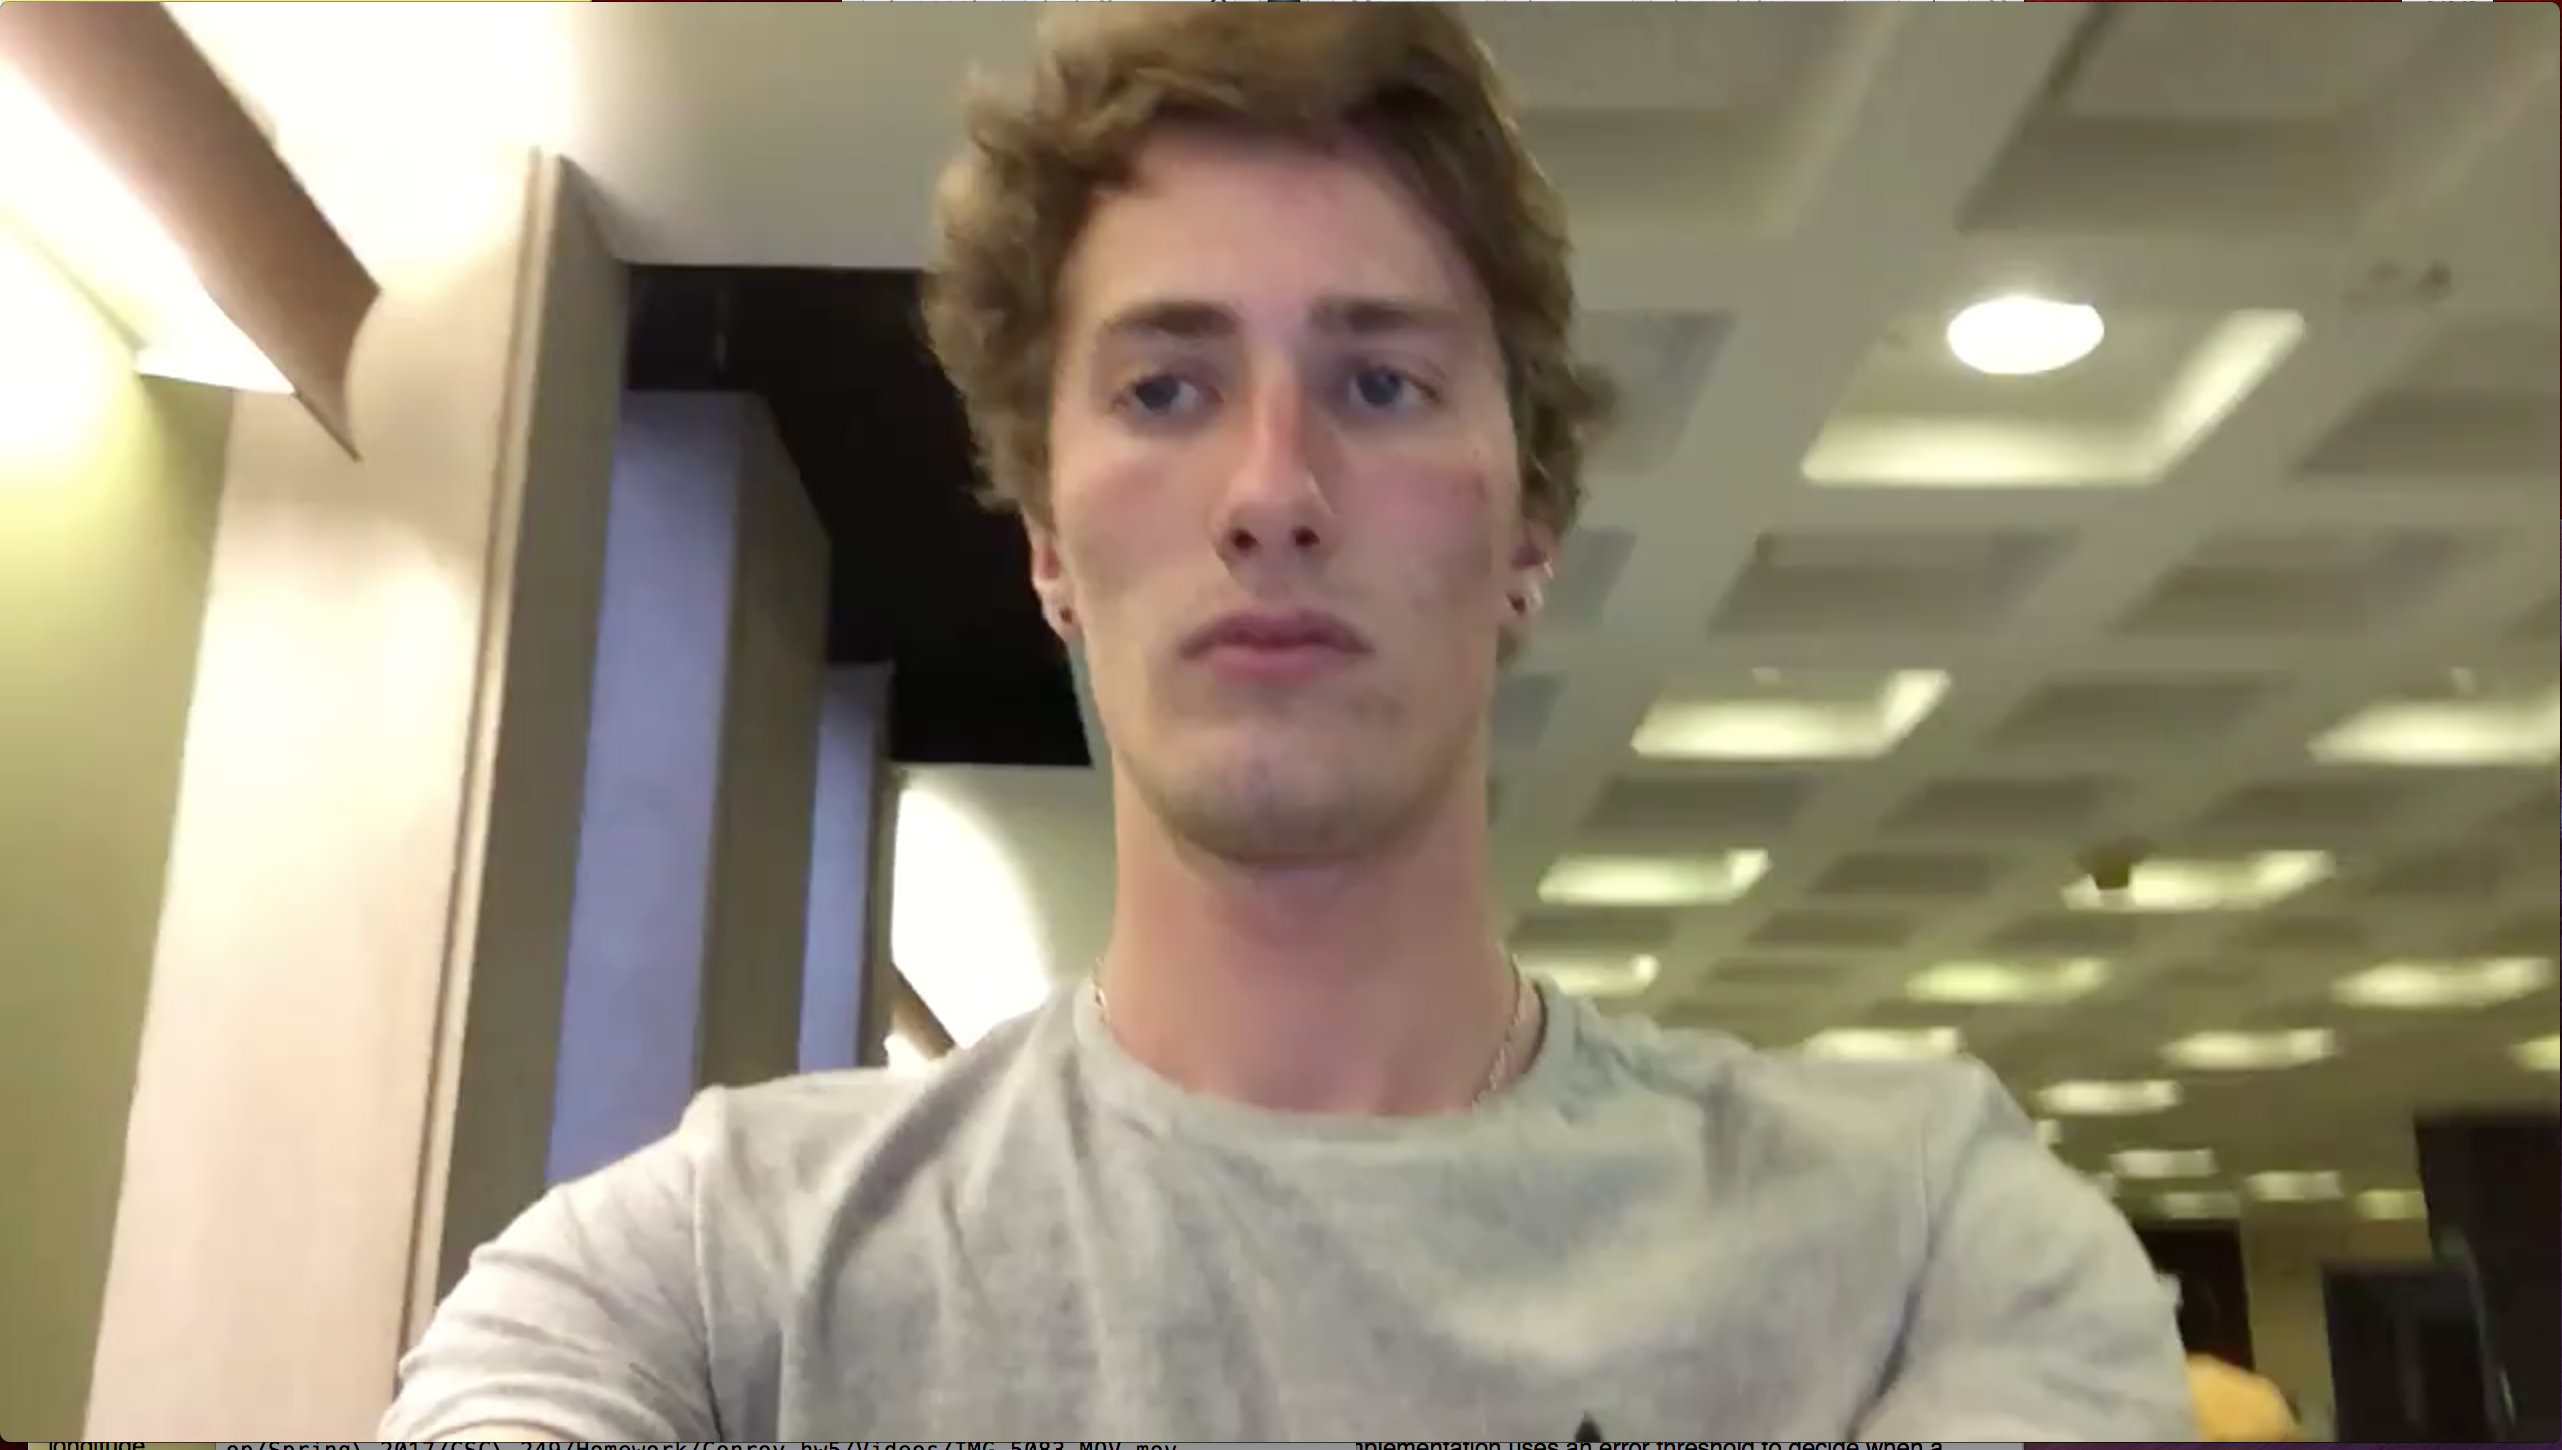
\includegraphics[width=\textwidth]{original_1.png}
    \caption{screenshot from original video}
  \end{minipage}
\end{figure}

\section{Kalman Filter}

Kalman filtering is an algorithm which takes a collection of inputs for known measurements or variables that have been observed over time, and uses them to estimate unknown states or variables as time moves on. It is used in the field of machine vision to track the movement of targeted objects in videos from frame to frame as they move within the field of view. The algorithm involves a two step process which includes a prediction step and an update step. During the prediction step the filter creates estimates of the current state of an object given its known variables as well as their uncertainties. During the update step, the next measurement is used to update the previous estimates by calculating a weighted average, with more weight being given to measurements with a higher degree of certainty.

For this task, I used an implementation that I found on GitHub which uses three features to model the tracking object: hue, saturation, and rotation invariant local binary pattern. Because the tracking heavily relies on color attributes, the bounding box stays focused on not only my face but my neck throughout the video.

This implementation seemed to perform a bit less smooth as the TLD overall. The bounding box wasn't as tight to my face, as it expanded to parts of my neck (see figure 2.1). However, the algorithm did seem to handle the rotation of my face better than the TLD, primarily because it was focusing on the hue and saturation of my skin tone and wasn't very disrupted by the event of some of my facial features leaving the frame (see figure 2.2).

\begin{figure}[H]
  \centering
  \begin{minipage}[b]{0.7\textwidth}
    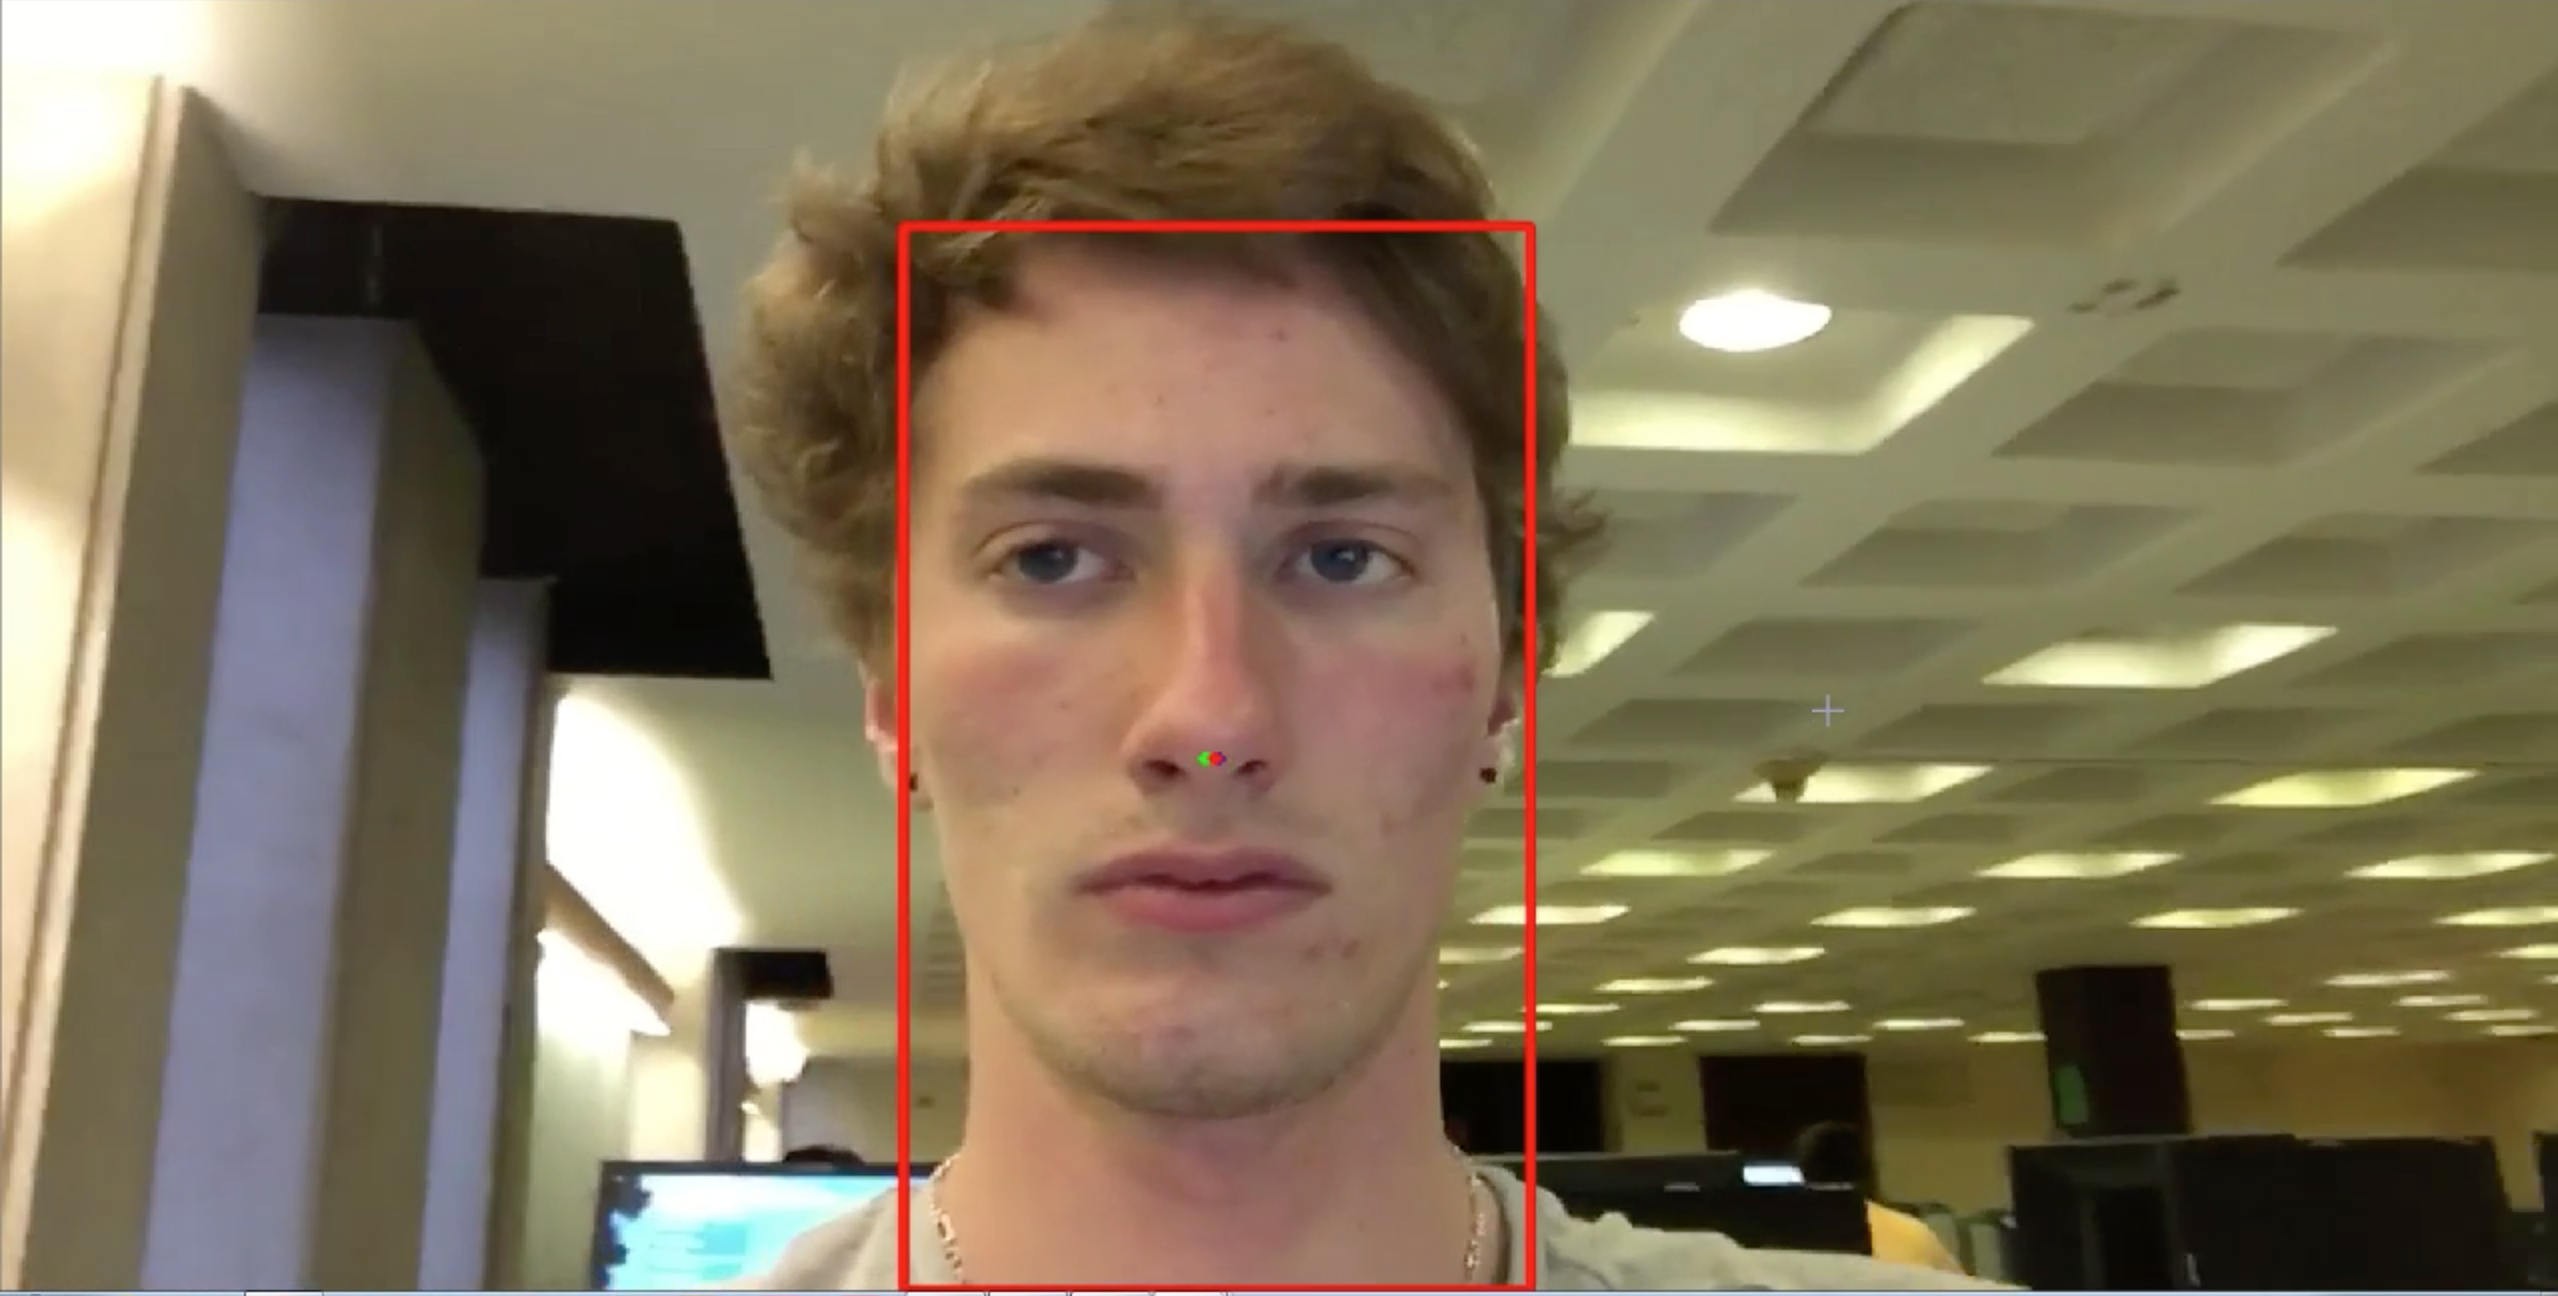
\includegraphics[width=\textwidth]{kalman_1.png}
    \caption{Kalman filter tracking face and neck}
  \end{minipage}
\end{figure}

\begin{figure}[H]
  \centering
  \begin{minipage}[b]{0.7\textwidth}
    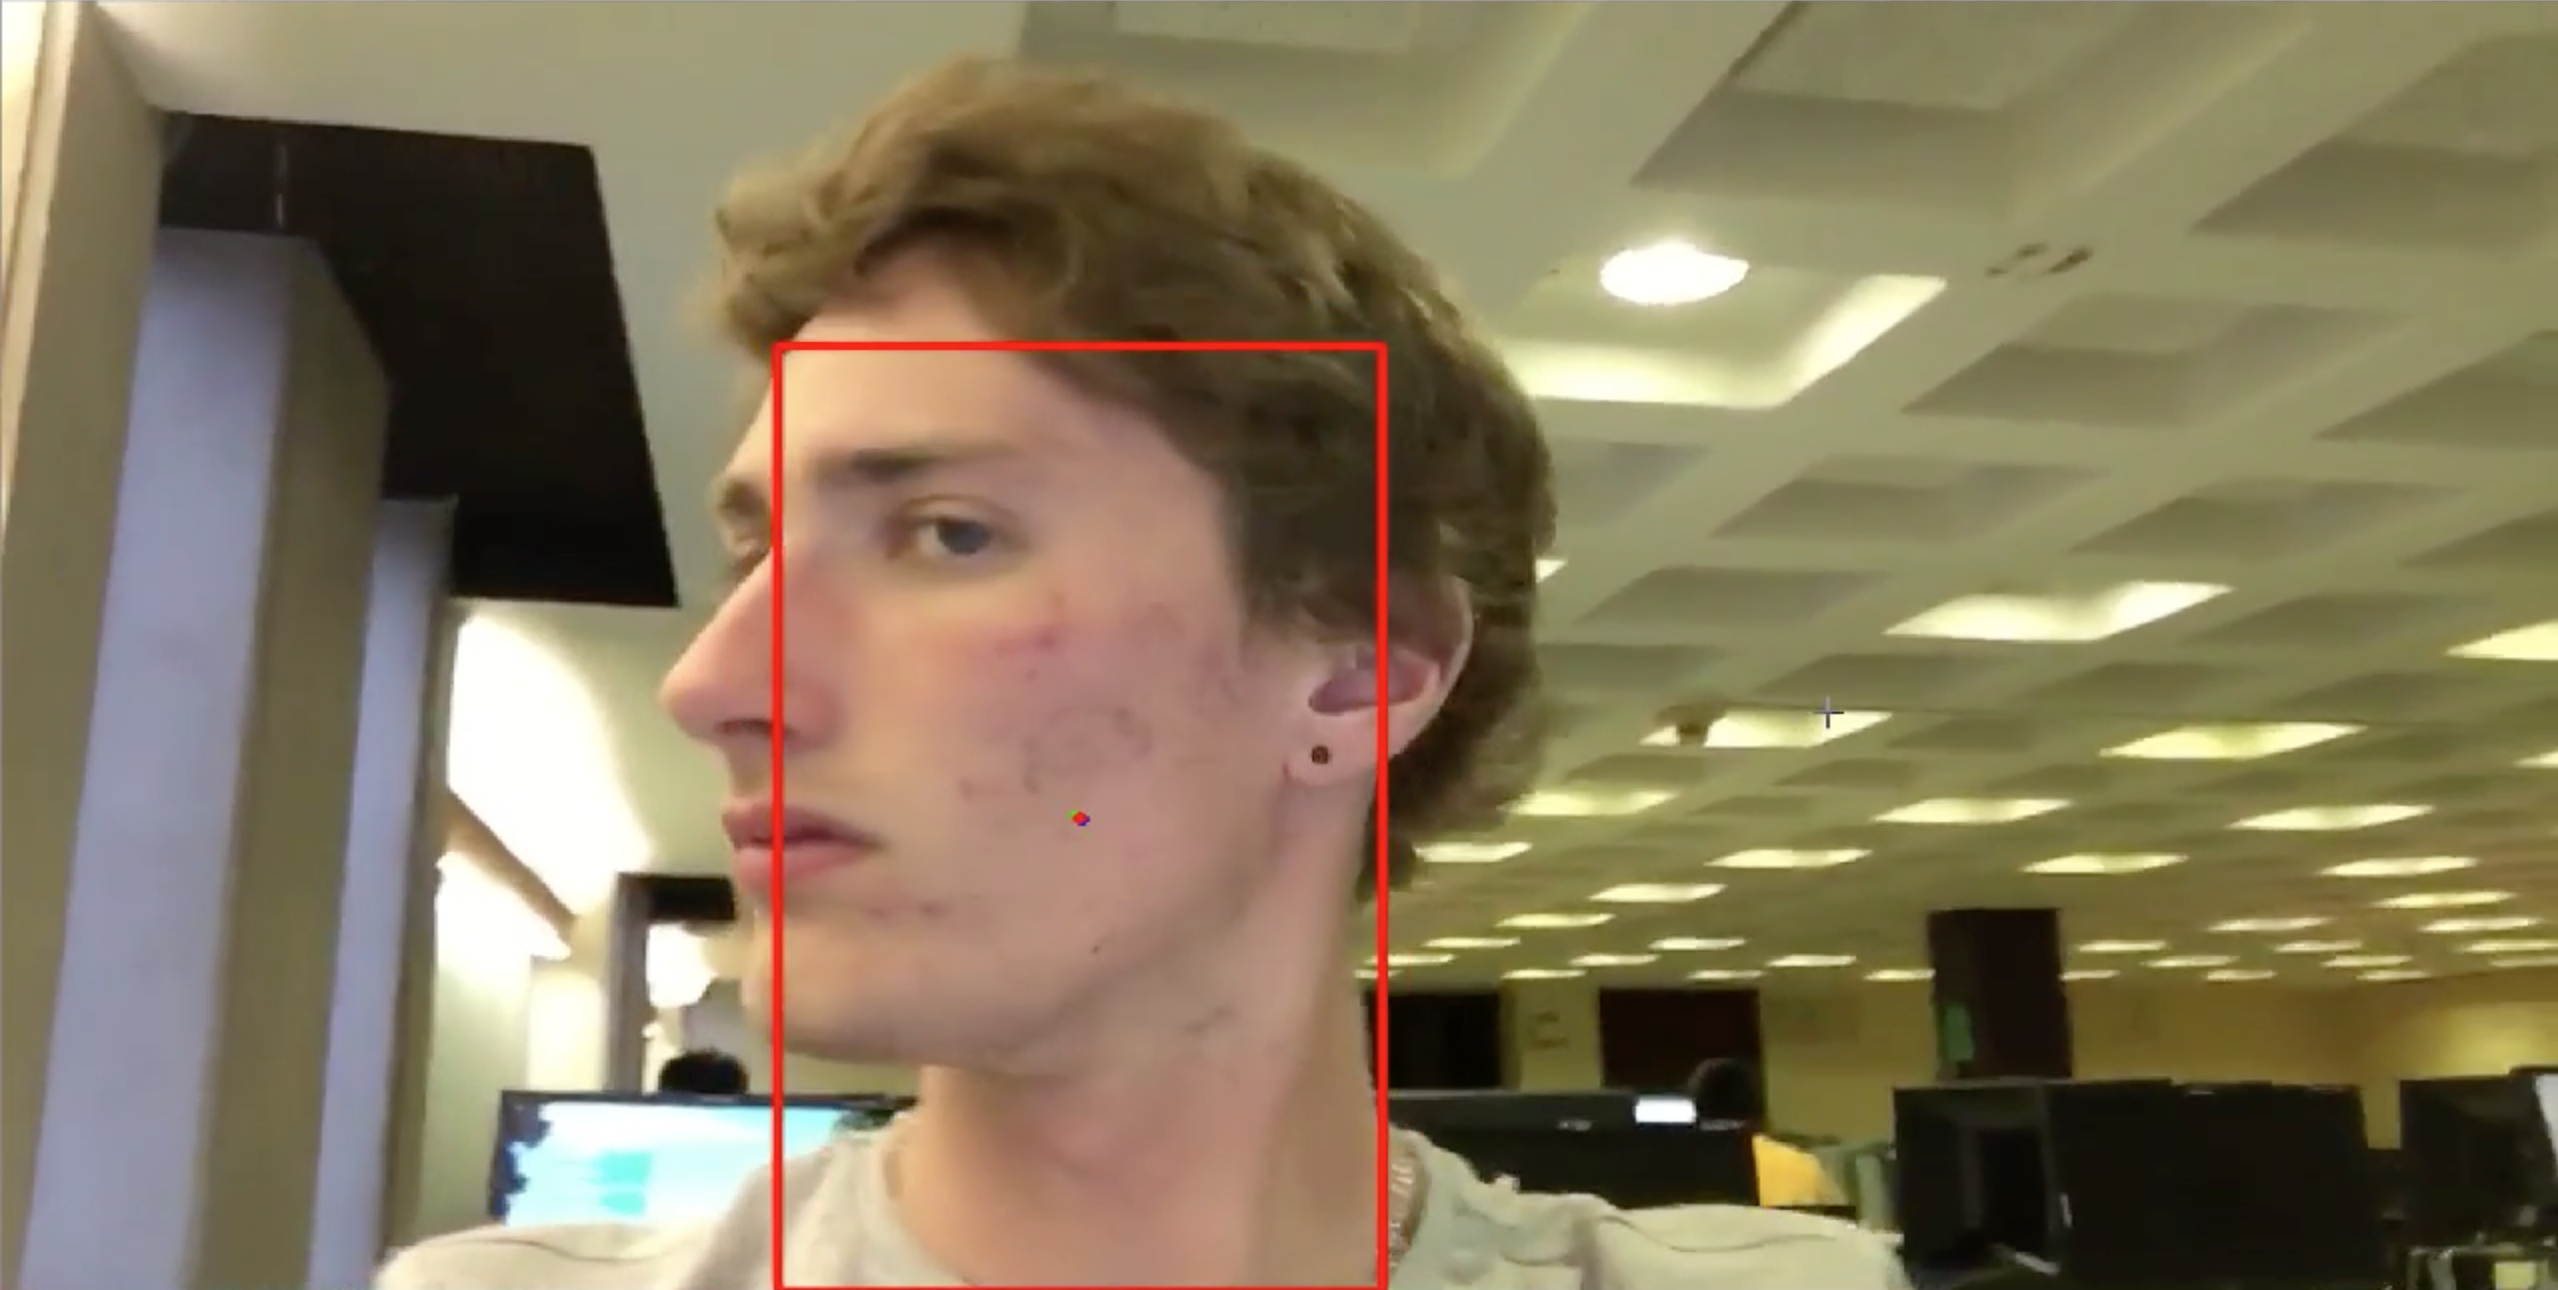
\includegraphics[width=\textwidth]{kalman_2.png}
    \caption{tracking my face turned to the side}
  \end{minipage}
\end{figure}

\section{TLD}

TLD tracking breaks up the process of tracking an object into 3 subtasks which work concurrently. The subtasks are tracking, learning, and detection. Tracking is the process of following an object from frame to frame, the detecting process involves looking at all of the appearances of the targeted object that have happened up to the current point in time and adjusts the tracker if it strays, and the learning process detects errors that have been made by the tracker and uses estimations to avoid these errors going forward.

For this task, I used an implementation that I found on GitHub which uses a recursive tracking algorithm that estimates the location of an array of points within a bounding box that is specified in the first frame from their position in the last frame. The implementation uses an error threshold to decide when a bounding box should be abandoned and reinitialized, such as when there is an occlusion blocking the target object. The detection is implemented by splitting up the video area into many small subwindows which are evaluated using a sliding window approach to check if the subwindow contains the target object. The subwindows are first discriminated by foreground and background, so that the background area is not within the search space and therefore not considered for evaluation.

The implementation seemed to perform very smoothly as seen in the video. I gave the initial boundaries for my face in the first frame as I launched the program. As my full face stays within the video frame, the  boundary box stays locked in with a high level of accuracy as seen in figure 3.1. The only time that the algorithm really "lost" my face was when I turned to the side, and half of my face left the frame (figures 3.2 and 3.3). Although, as my full face re-entered the frame, the bounding box reinitialized and found my face again (figure 3.4).

\begin{figure}[H]
  \centering
  \begin{minipage}[b]{0.7\textwidth}
    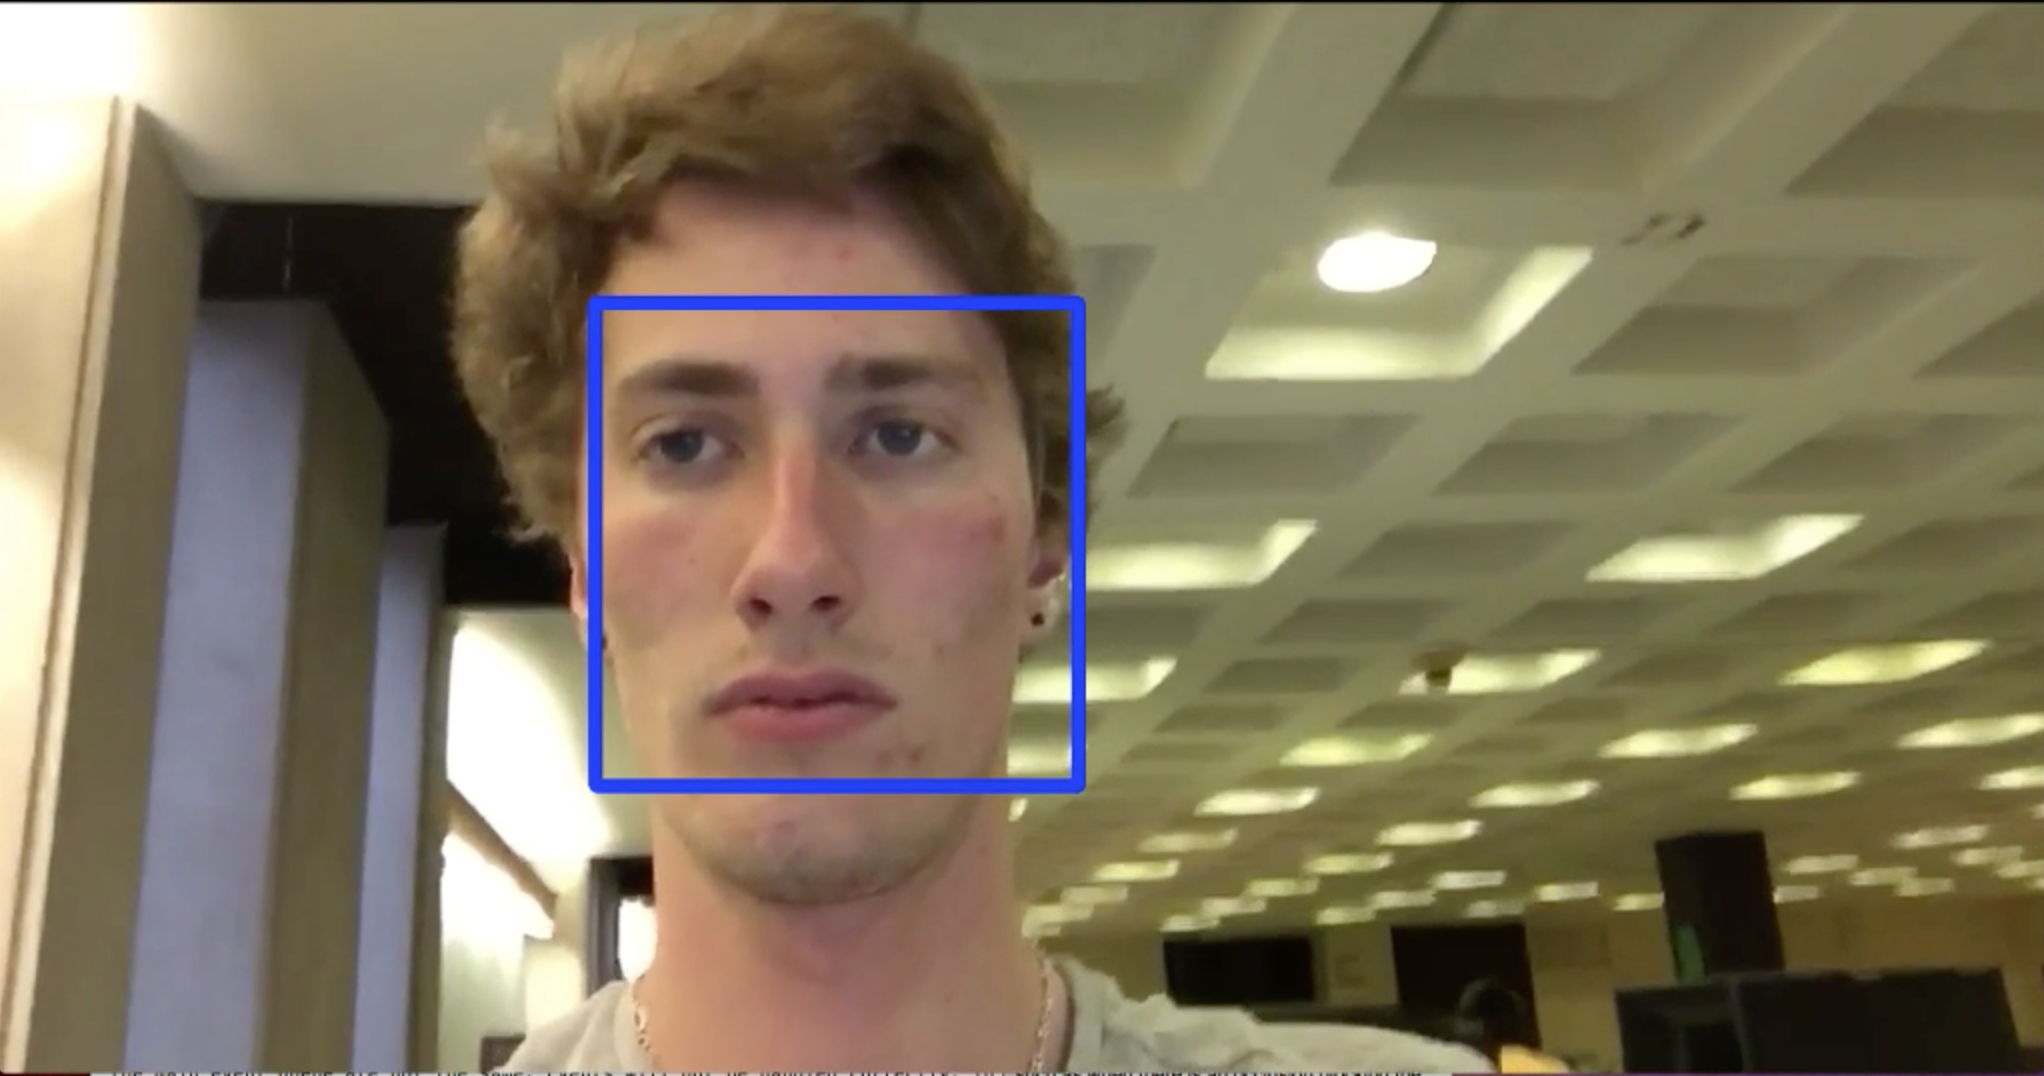
\includegraphics[width=\textwidth]{tld_1.png}
    \caption{TLD tracking my face}
  \end{minipage}
\end{figure}

\begin{figure}[H]
  \centering
  \begin{minipage}[b]{0.7\textwidth}
    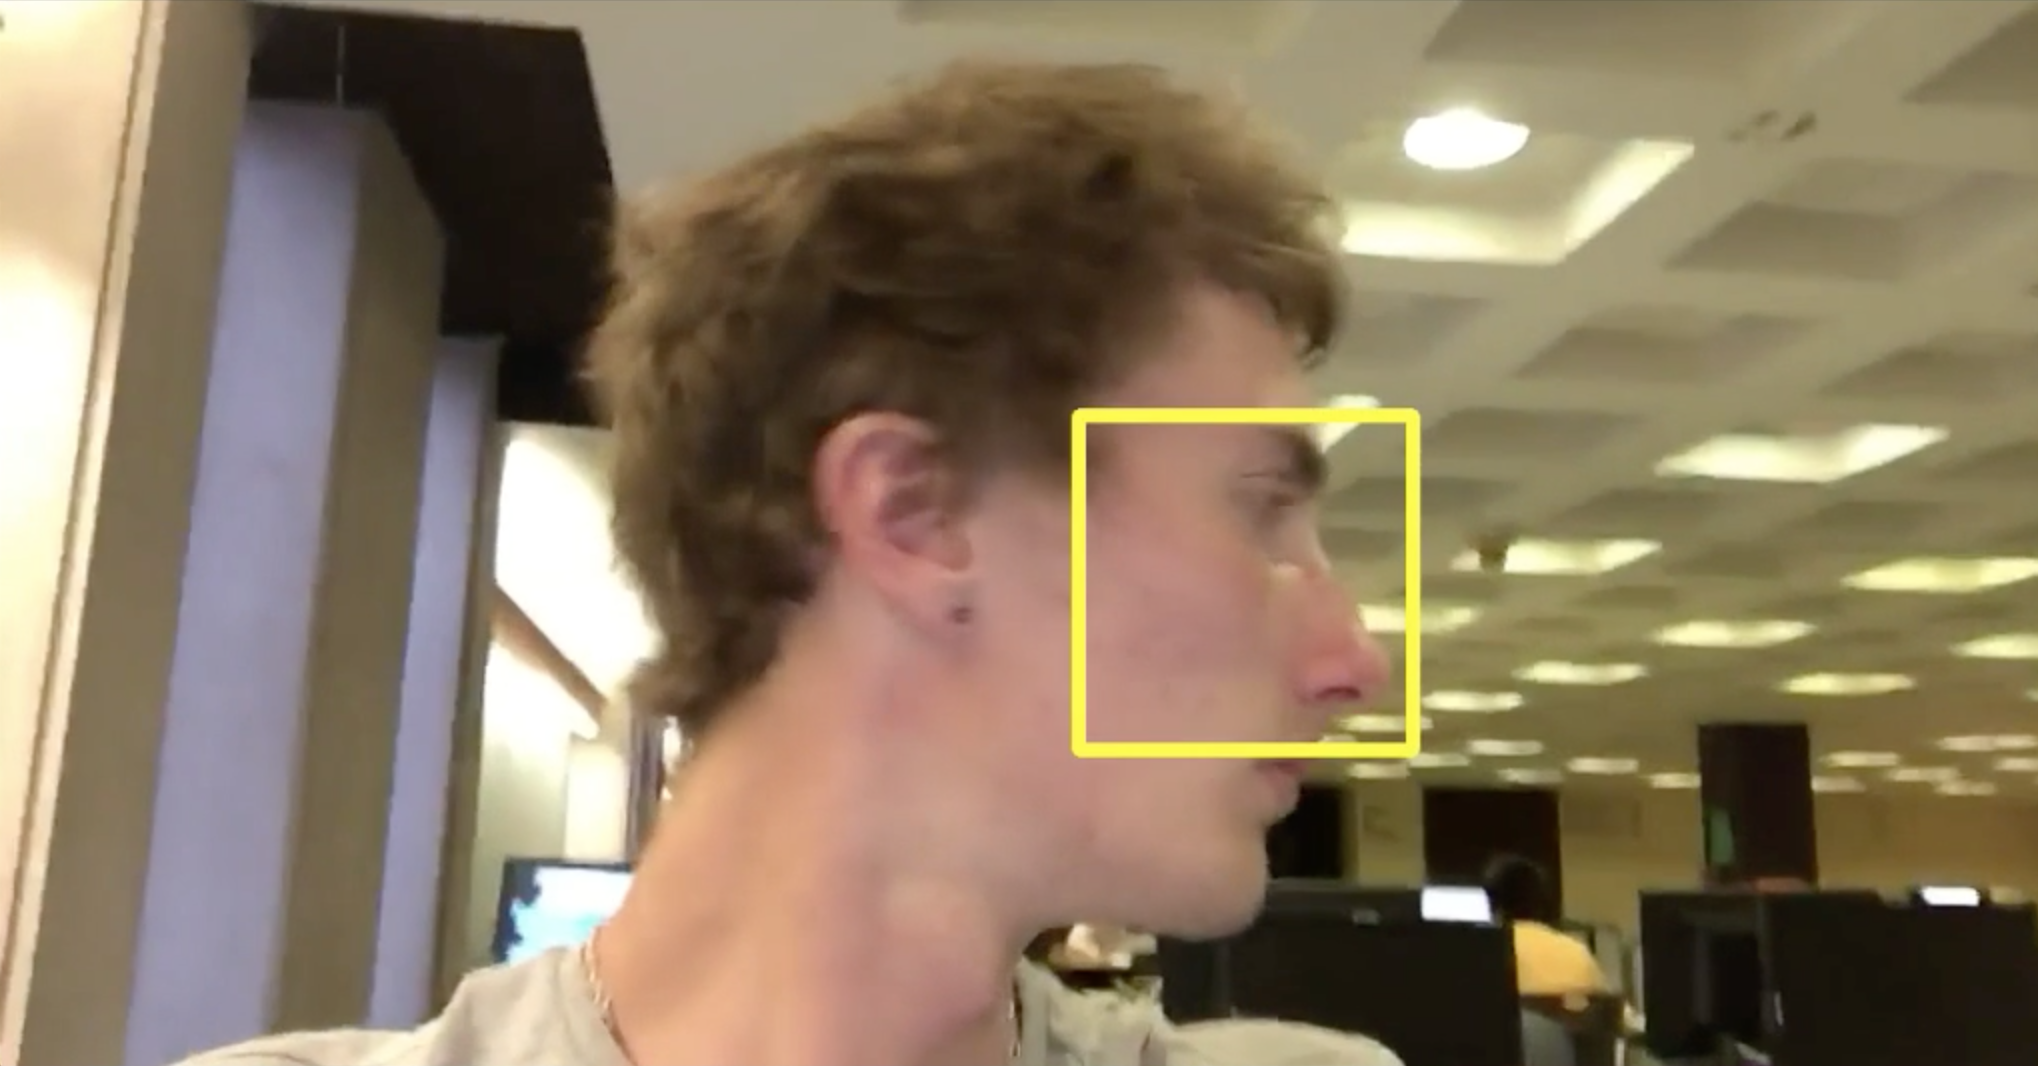
\includegraphics[width=\textwidth]{tld_2.png}
    \caption{tracking is disrupted as I turn my head}
  \end{minipage}
\end{figure}

\begin{figure}[H]
  \centering
  \begin{minipage}[b]{0.7\textwidth}
    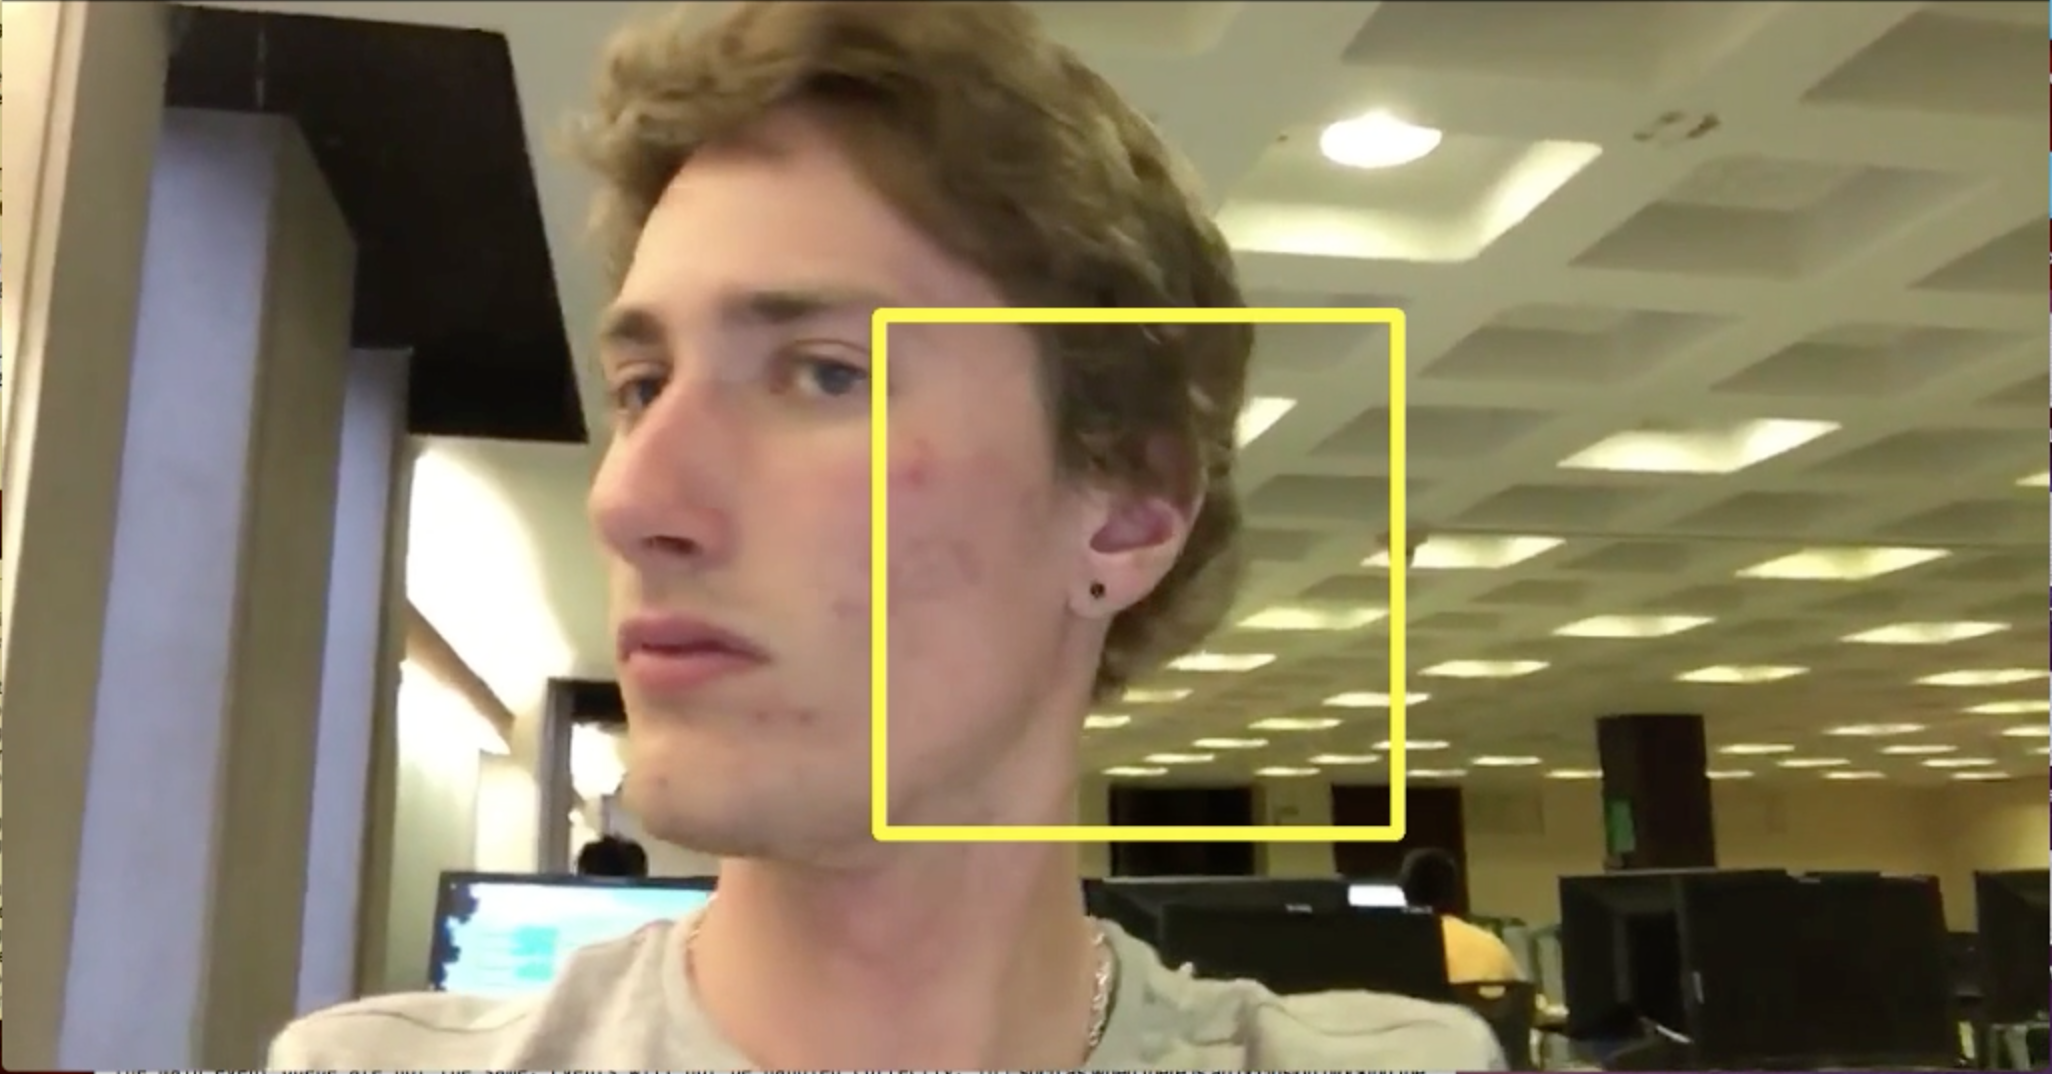
\includegraphics[width=\textwidth]{tld_3.png}
    \caption{tracking is disrupted as I turn my head}
  \end{minipage}
\end{figure}

\begin{figure}[H]
  \centering
  \begin{minipage}[b]{0.7\textwidth}
    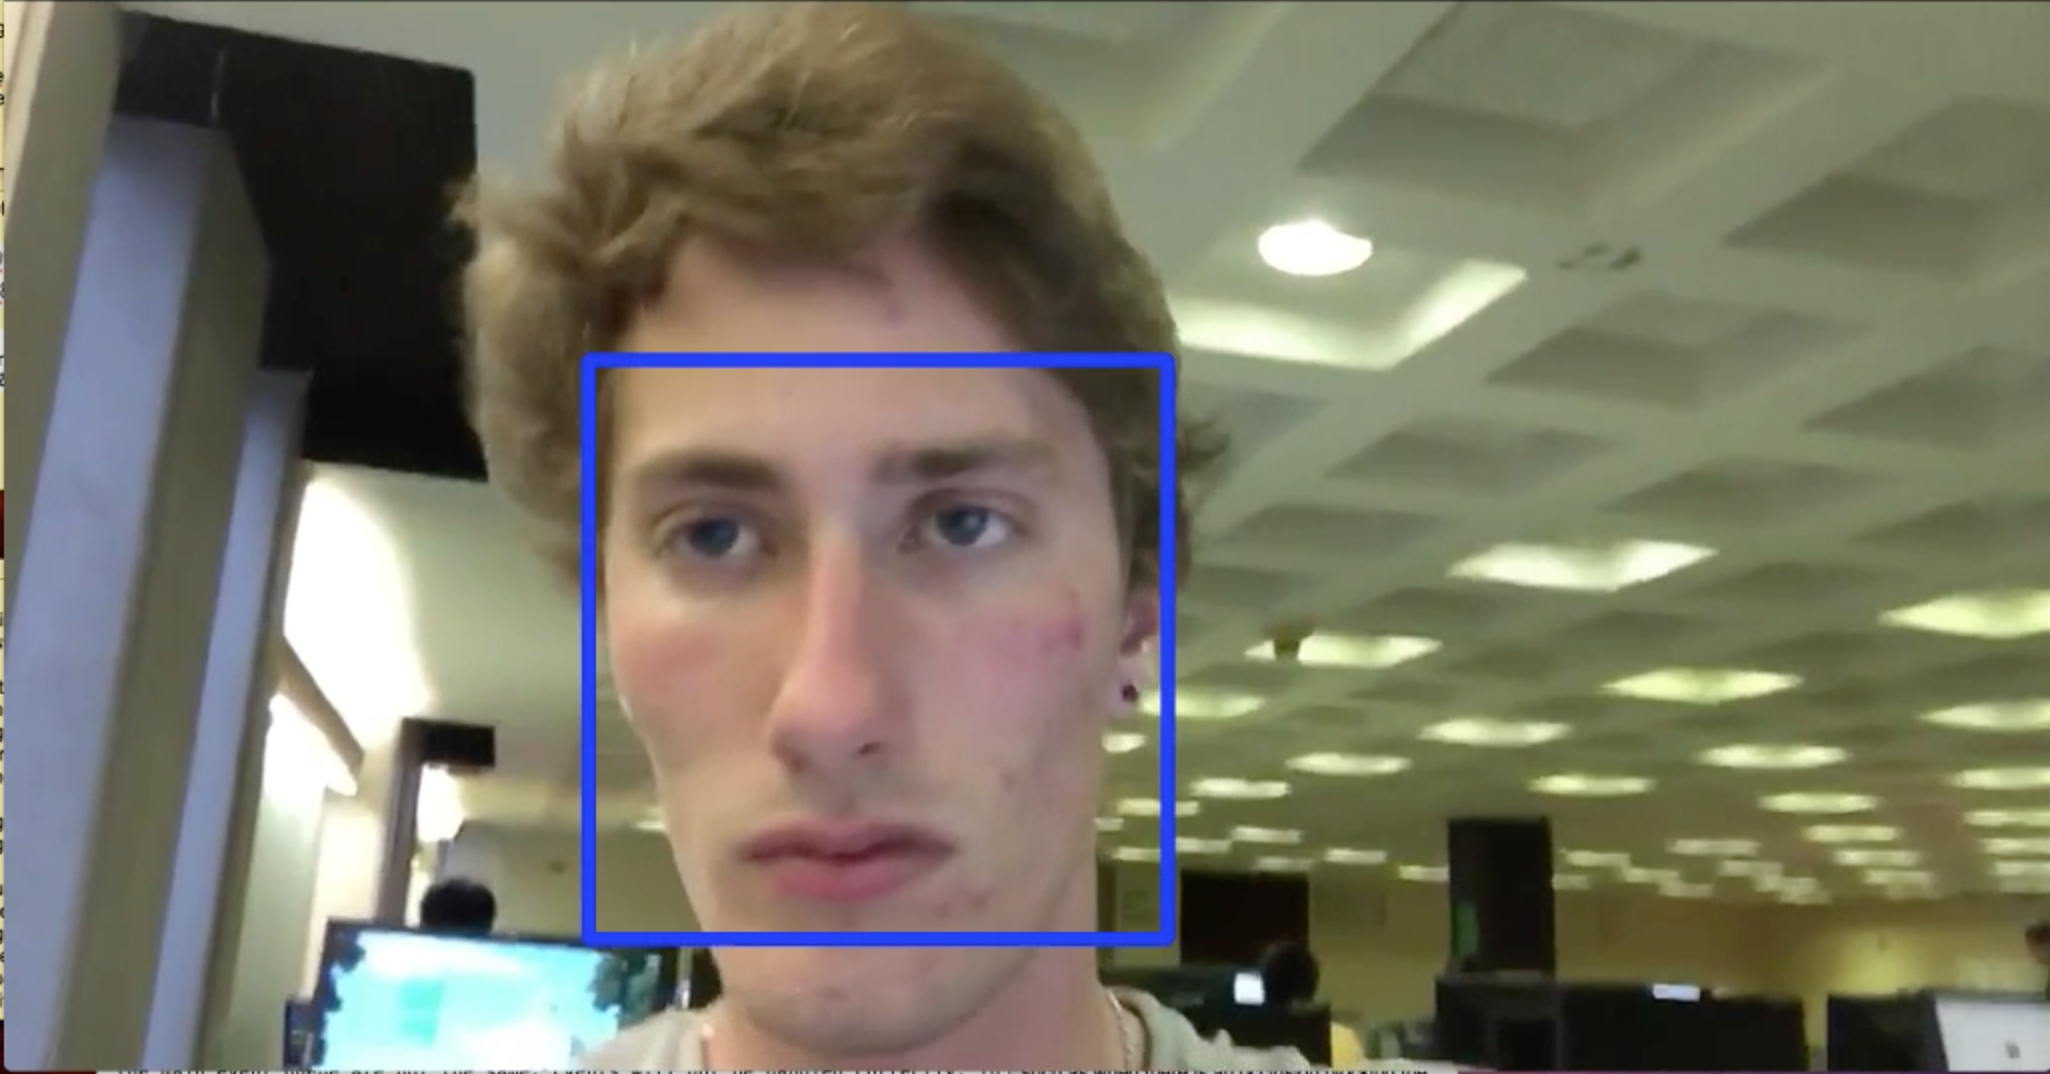
\includegraphics[width=\textwidth]{tld_4.png}
    \caption{TLD reinitializes bounding box, finds face again}
  \end{minipage}
\end{figure}

\section{Videos}

My recorded videos can be found in the "Videos" directory.

\begin{itemize}
  \item original.mov -- the original video
  \item kalman.mov -- a video of the Kalman filter tracking my face
  \item tld.mov -- a video of the TLD tracking my face
\end{itemize}

\section{Sources}

Cheng, Shaoguang, camshiftKalman, (2015), GitHub repository, https://github.com/shaoguangcheng/-camshiftKalman

Nebehay, Georg, open\textunderscore tld, (2015), GitHub repository, https://github.com/pandora-auth-ros-pkg/open\textunderscore tld

\end{document}